\section{The problem}\label{sec:problem}

A cross-country flight alternates three phases (Figure~\ref{fig:flight}), the
transition--search--climb cycle of~\cite{vilpellet2026}:
\begin{itemize}
  \item \textcolor{transition}{\textbf{transition}}: the pilot glides from one thermal towards the
        next; the track is nearly straight and sinks;
  \item \textcolor{search}{\textbf{search}}: there is no lift where the pilot expected it; the pilot
        turns, probes and changes heading; the track bends without a settled direction and the
        height changes little;
  \item \textcolor{climb}{\textbf{climb}}: in a thermal the pilot circles, always turning the same
        way, and rises.
\end{itemize}
Labelling every fix with its phase gives the statistics of each phase: how long climbs last, how
far glides go, how much time a pilot spends searching.

\begin{figure}
\centering
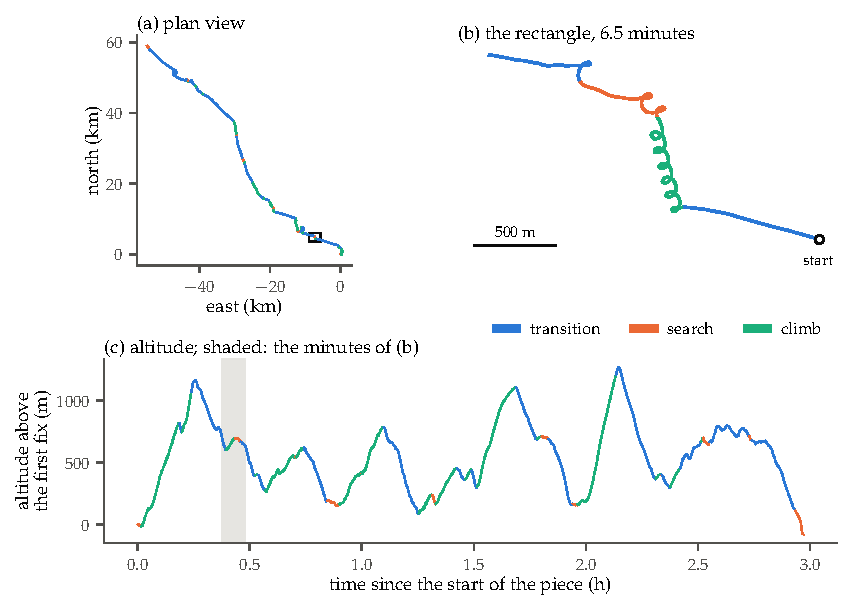
\includegraphics[width=\textwidth]{figures/flight_phases.pdf}
\caption{A 3-hour paraglider flight labelled by the method at 1~Hz. (a) Plan view; the rectangle
is panel (b). (b) 6.5 minutes of it: a glide, a climb that drifts with the wind, a search, and a
glide again. (c) GNSS altitude above the first fix of the piece: the climbs are the rising
stretches; the shaded band marks the minutes of (b), within the 24 minutes of
Figure~\ref{fig:features}.}
\label{fig:flight}
\end{figure}

Two things make the labelling hard. Nobody has labelled the fixes by hand, and the phases are only
partly objective: the end of a glide and the start of a search have no sharp boundary. And a GNSS
fix wobbles by a few metres, enough to fake a turn at one fix per second. Vilpellet answers both
in two stages: simple yes/no features computed over 30~s absorb the wobble, and a hidden Markov
model picks the phase sequence that best explains the features while making each change of phase
costly.

\paragraph{Logging intervals.} The model was fitted on tracks logged once per second. Table~\ref{tab:cadence}
shows how many flights of the archive are logged at another interval: one paraglider flight in
three, and seven hang-glider flights in ten. Section~\ref{sec:cadence} is about them.

\begin{table}
\centering
\small
\begin{tabular}{@{}l r *{7}{r}@{}}
\toprule
 & flights & 1~s & 2~s & 3~s & 4~s & 5~s & 10~s & other \\
\midrule
paragliders & 185\,321 & 69.6\% & 9.5\% & 5.1\% & 2.2\% & 9.7\% & 2.4\% & 1.5\% \\
hang gliders & 6\,536 & 30.4\% & 13.5\% & 9.6\% & 3.0\% & 26.6\% & 15.2\% & 1.7\% \\
\bottomrule
\end{tabular}
\caption{Logging interval of the FFVL flights that pass the altitude and speed rules of the
xc-dynamics pre-processing (column \texttt{sampling\_s} of
\texttt{derived/preprocessing/vertical/flights.csv}).}
\label{tab:cadence}
\end{table}
